

%  article.tex (Version 3.3, released 19 January 2008)
%  Article to demonstrate format for SPIE Proceedings
%  Special instructions are included in this file after the
%  symbol %>>>>
%  Numerous commands are commented out, but included to show how
%  to effect various options, e.g., to print page numbers, etc.
%  This LaTeX source file is composed for LaTeX2e.

%  The following commands have been added in the SPIE class 
%  file (spie.cls) and will not be understood in other classes:
%  \supit{}, \authorinfo{}, \skiplinehalf, \keywords{}
%  The bibliography style file is called spiebib.bst, 
%  which replaces the standard style unstr.bst.  

\documentclass[a4paper]{spie}  %>>> use for US letter paper
%%\documentclass[a4paper]{spie}  %>>> use this instead for A4 paper
%%\documentclass[nocompress]{spie}  %>>> to avoid compression of citations
%% \addtolength{\voffset}{9mm}   %>>> moves text field down
%% \renewcommand{\baselinestretch}{1.65}   %>>> 1.65 for double spacing, 1.25 for 1.5 spacing 
%  The following command loads a graphics package to include images 
%  in the document. It may be necessary to specify a DVI driver option,
%  e.g., [dvips], but that may be inappropriate for some LaTeX 
%  installations. 
\usepackage{amsmath}
\usepackage[]{graphicx}
\usepackage{hyperref}
\usepackage{listings}
\hypersetup{
    colorlinks,
    linkcolor={black!50!black},
    citecolor={blue!50!black},
    urlcolor={blue!80!black}
}
\usepackage{pdfpages}
\usepackage{parcolumns}

\usepackage[utf8]{inputenc} 
\usepackage[ngerman]{babel}
\usepackage[autostyle=true,german=quotes]{csquotes}

\usepackage{color}
\definecolor{lightgray}{rgb}{.9,.9,.9}
\definecolor{darkgray}{rgb}{.4,.4,.4}
\definecolor{purple}{rgb}{0.65, 0.12, 0.82}


\usepackage{array}
\newcolumntype{L}[1]{>{\raggedright\let\newline\\\arraybackslash\hspace{0pt}}m{#1}}
\newcolumntype{C}[1]{>{\centering\let\newline\\\arraybackslash\hspace{0pt}}m{#1}}
\newcolumntype{R}[1]{>{\raggedleft\let\newline\\\arraybackslash\hspace{0pt}}m{#1}}

\usepackage{xcolor,colortbl}
\usepackage{color}
\usepackage{float}

\title{Smartphonecontroller Javascript-GameAPI}

%>>>> The author is responsible for formatting the 
%  author list and their institutions.  Use  \skiplinehalf 
%  to separate author list from addresses and between each address.
%  The correspondence between each author and his/her address
%  can be indicated with a superscript in italics, 
%  which is easily obtained with \supit{}.

\author{ Ron Schiwkowksi  (918691), Hannes Grothknopf (915449), Michael Schleiss (923739), Christian Heinrichs (919020), Dennis Hofmann (919285)
\skiplinehalf
University of Applied Sciences, Sokratesplatz 1, 24149 Kiel, Germany
}

%%%%%%%%%%%%%%%%%%%%%%%%%%%%%%%%%%%%%%%%%%%%%%%%%%%%%%%%%%%%% 
%>>>> uncomment following for page numbers
\pagestyle{plain}    
%>>>> uncomment following to start page numbering at 301 
%\setcounter{page}{301} 
 
  \begin{document} 
  \maketitle 
%%%%%%%%%%%%%%%%%%%%%%%%%%%%%%%%%%%%%%%%%%%%%%%%%%%%%%%%%%%%% 
\begin{abstract}
Lorem ipsum dolor sit amet, consetetur sadipscing elitr, sed diam nonumy eirmod tempor invidunt ut labore et dolore magna aliquyam erat, sed diam voluptua. At vero eos et accusam et justo duo dolores et ea rebum. Stet clita kasd gubergren, no sea takimata sanctus est Lorem ipsum dolor sit amet. Lorem ipsum dolor sit amet, consetetur sadipscing elitr, sed diam nonumy eirmod tempor invidunt ut labore et dolore magna aliquyam erat, sed diam voluptua. At vero eos et accusam et justo duo dolores et ea rebum. Stet clita kasd gubergren, no sea takimata sanctus est Lorem ipsum dolor sit amet.
\end{abstract}

%>>>> Include a list of keywords after the abstract 
\keywords{Smartphone, JavaScript, HTML5, Nodejs, API}

%%%%%%%%%%%%%%%%%%%%%%%%%%%%%%%%%%%%%%%%%%%%%%%%%%%%%%%%%%%%%
\section{Einleitung}
Lorem ipsum dolor sit amet, consetetur sadipscing elitr, sed diam nonumy eirmod tempor invidunt ut labore et dolore magna aliquyam.

\subsection{Problemstellung}
Lorem ipsum dolor sit amet, consetetur sadipscing elitr, sed diam nonumy eirmod tempor invidunt ut labore et dolore magna aliquyam erat, sed diam voluptua. At vero eos et accusam et justo duo dolores et ea rebum. Stet clita kasd gubergren, no sea takimata sanctus est Lorem ipsum dolor sit amet. Lorem ipsum dolor sit amet, consetetur sadipscing elitr, sed diam.
\begin{figure}[h!]
	\centering
		\fbox{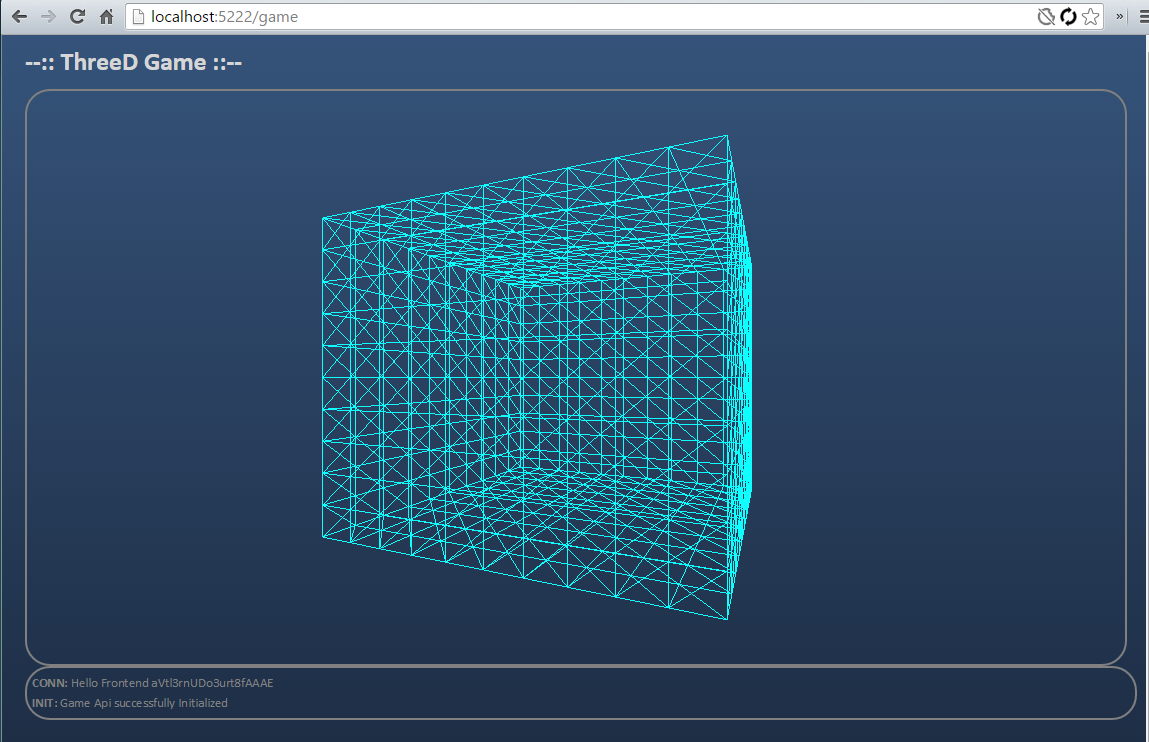
\includegraphics[width=12cm]{./images/FrontendInit.png}}
		\caption{Nicht ausgelastet Bar}
		\label{fig:FrontendInit}
\end{figure}

Lorem ipsum dolor sit amet, consetetur sadipscing elitr, sed diam nonumy eirmod tempor invidunt ut labore et dolore magna aliquyam erat, sed diam voluptua. At vero eos et accusam et justo duo dolores et ea rebum. Stet clita kasd gubergren, no sea takimata sanctus est Lorem ipsum dolor sit amet. Lorem ipsum dolor sit amet, consetetur sadipscing elitr, sed diam nonumy eirmod tempor invidunt ut labore et dolore magna aliquyam erat, sed diam voluptua. At vero eos et accusam et justo duo dolores et ea rebum. Stet clita kasd gubergren, no sea takimata sanctus est Lorem ipsum dolor sit amet.(siehe Abbildung \ref{fig:FrontendInit}).
\\
Lorem ipsum dolor sit amet, consetetur sadipscing elitr, sed diam nonumy eirmod tempor invidunt ut labore et dolore magna aliquyam erat, sed diam voluptua. At vero eos et accusam et justo duo dolores et ea rebum. Stet clita kasd gubergren, no sea takimata sanctus est Lorem ipsum dolor sit amet. Lorem ipsum dolor sit amet, consetetur sadipscing elitr, sed diam.

\section{Methods}
\subsection{Projektmanagement}
Die Verteilung der Aufgaben ist in Tabelle \ref{table:distribution of tasks} aufgestellt.
Aufgaben sind im Gitlab erfasst und Personen zugewiesen. Ein wöchentliches persönliches Treffen aller Projektmitglieder führt zu einer guten Arbeitsmoral und hohen Effektivität.
\paragraph{GitLab}
Das Proket wurde auf einem eigenen GitLab gehostet und den Projektmitgliedern zur Verfügung gestellt. Die Issues wurden genutzt um Aufgaben zu Verteilung und zu dokumentieren.
Strukuriert wurde das Arbeiten nach Feature Branches, um das Arbeiten am Projekt möglichst flexibel zu halten. Der Master-Branch diente als Release-Branch, in den regelmäßig die Änderungen per Merge Request eingetragen und getestet wurden.
\definecolor{blau}{HTML}{217AA2}
\begin{table}
	\label{table:distribution of tasks}
	\centering
		\caption{Matrix distribution of tasks}
		\begin{tabular}{| L{2.6cm} | C{2cm} | C{2cm} | C{2cm} | C{2cm} | C{2cm} |}
		\hline
		\rowcolor{blau}
		\textcolor{white}{\textbf{Aufgabe}} & \textcolor{white}{\textbf{Schleiss}} & \textcolor{white}{\textbf{Grothknopf}} & \textcolor{white}{\textbf{Schiwkowksi}} & \textcolor{white}{\textbf{Hofmann}} & \textcolor{white}{\textbf{Heinrichs}}\\\hline
		Recherche 		& X & X	& X	& X	& X	\\\hline
		Konzept 		& X & X	& X	& X	& X	\\\hline
		Serverdesign	& 	& X & 	& X	& X \\\hline
		Networking		& 	& X	& 	& X	& X	\\\hline
		GameAPI 		& 	& X	&	&	& X	\\\hline
		DemoGame 		& X	&	&	&	& X	\\\hline
		ClientFrontend 	& X	&	& X	&	&	\\\hline
		ClientBackend 	& X	&	& X	&	&	\\\hline
		Database 	    & 	&	&	& X	& 	\\\hline
		LoginHandling   & 	& 	& 	& X	& 	\\\hline
		Poster          & 	& 	& 	& 	& 	\\\hline
		Documentation   & 	& 	& 	& 	& X \\\hline
		Projektmgmt. 	&	&	&	& 	& X	\\\hline
	\end{tabular} 
\end{table}

\subsection{Technologies}
\subsubsection{NodeJS}
Was ist NodeJS, Warum genutzt
\begin{figure}[h!]
	\centering
		\fbox{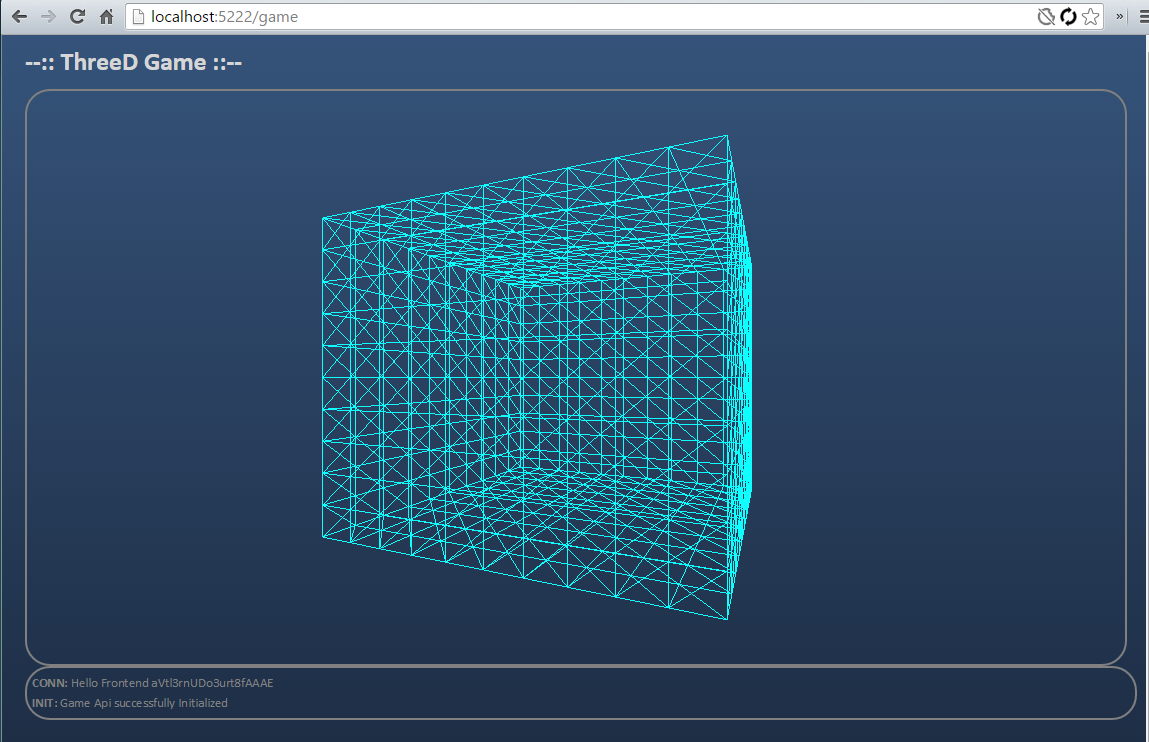
\includegraphics[width=12cm]{./images/FrontendInit.png}}
		\caption{Systemarchitektur WiFi Tracking}
		\label{fig:sysArch}
\end{figure}

Die Berechnung der Signalstärke wird nicht durch Kismet vorgenommen, sondern geschieht intern in der jeweiligen Netzwerkkarte. Es wird bei den Raspberry Pi ein LOGILINK WL0084B WiFi-USB-Stick verwendet. Die Dämpfung kann bei verschieden Netzwerkkarten stark abweichen. Deshalb ist es erforderlich, dass im Versuchsaufbau nur gleiche Netzwerkkarten verwendet werden.

\subsubsection{HTML 5}
Was kann HTML5, was nutzen wir für HTML 5 Features
\begin{figure}[h!]
	\centering
		\fbox{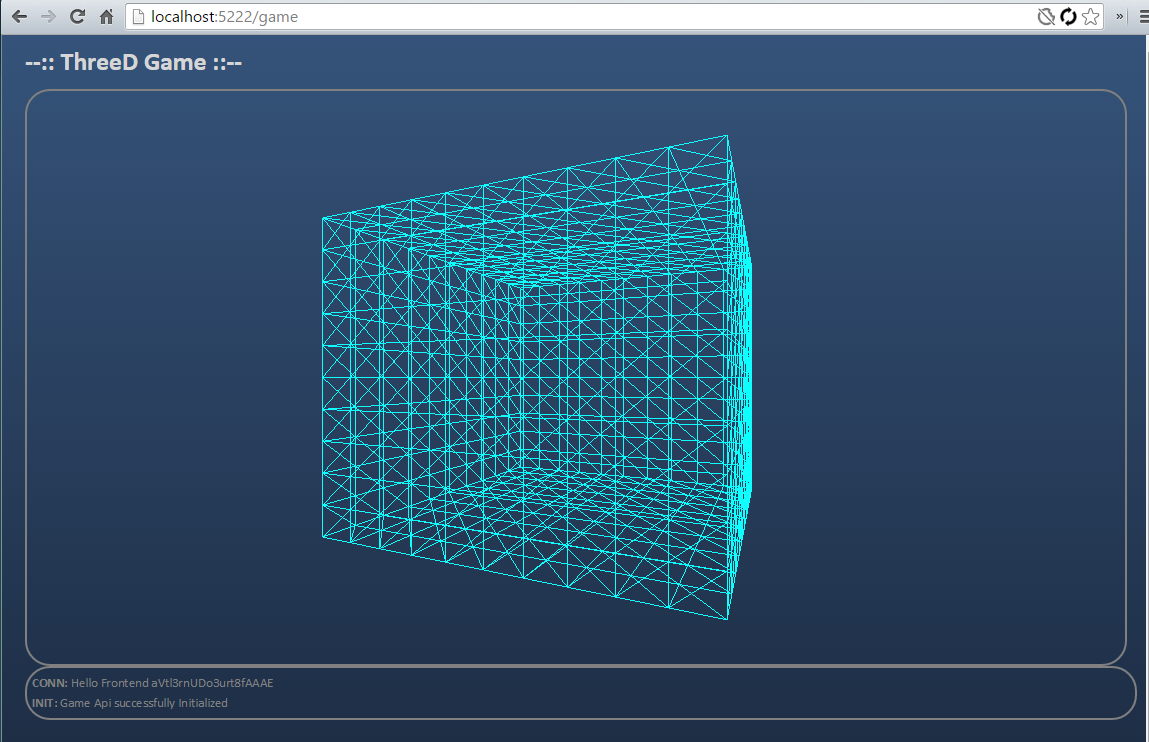
\includegraphics[width=10cm]{./images/FrontendInit.png}}
		\caption{Virtuelle Maschinen vs. Docker Container\cite{dockercontainer}}
		\label{fig:dockerVM}
\end{figure}

\subsubsection{Jacascript}
Was kann Javascript, ECMA 6
\begin{figure}[h!]
	\centering
		\fbox{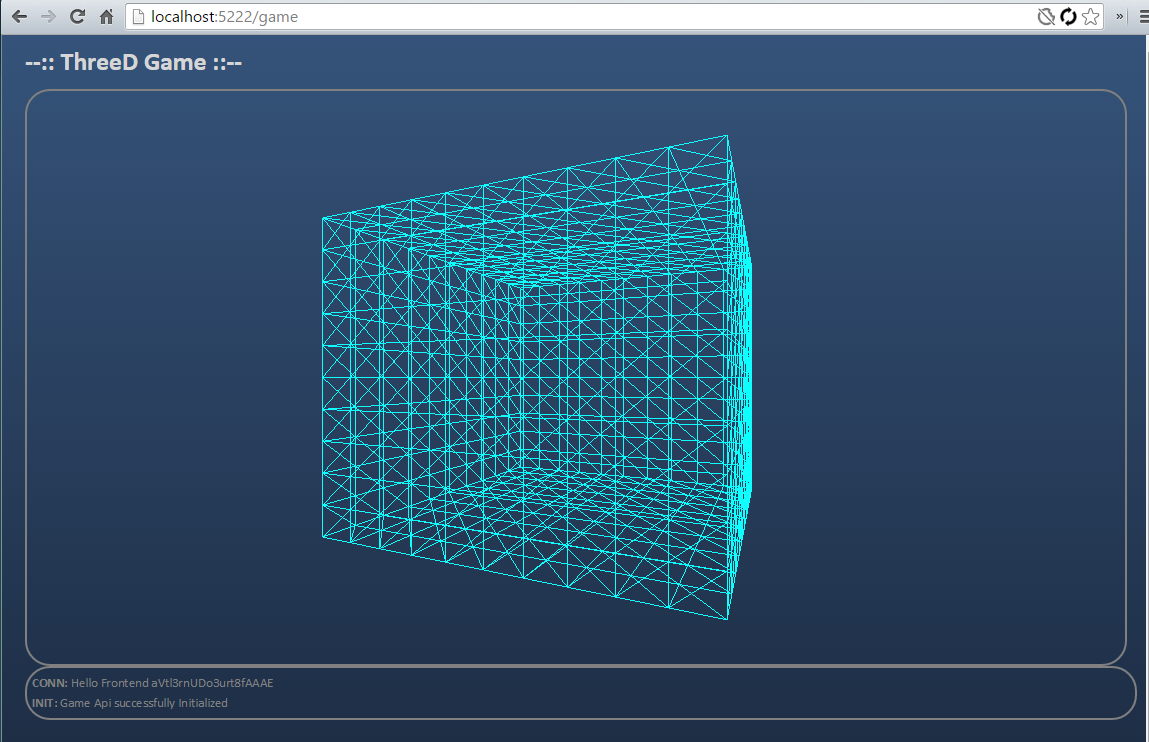
\includegraphics[width=10cm]{./images/FrontendInit.png}}
		\caption{Virtuelle Maschinen vs. Docker Container\cite{dockercontainer}}
		\label{fig:dockerVM}
\end{figure}
\subsubsection{MongoDB}
Was kann MongoDB, Warum MongoDB
\begin{figure}[h!]
	\centering
		\fbox{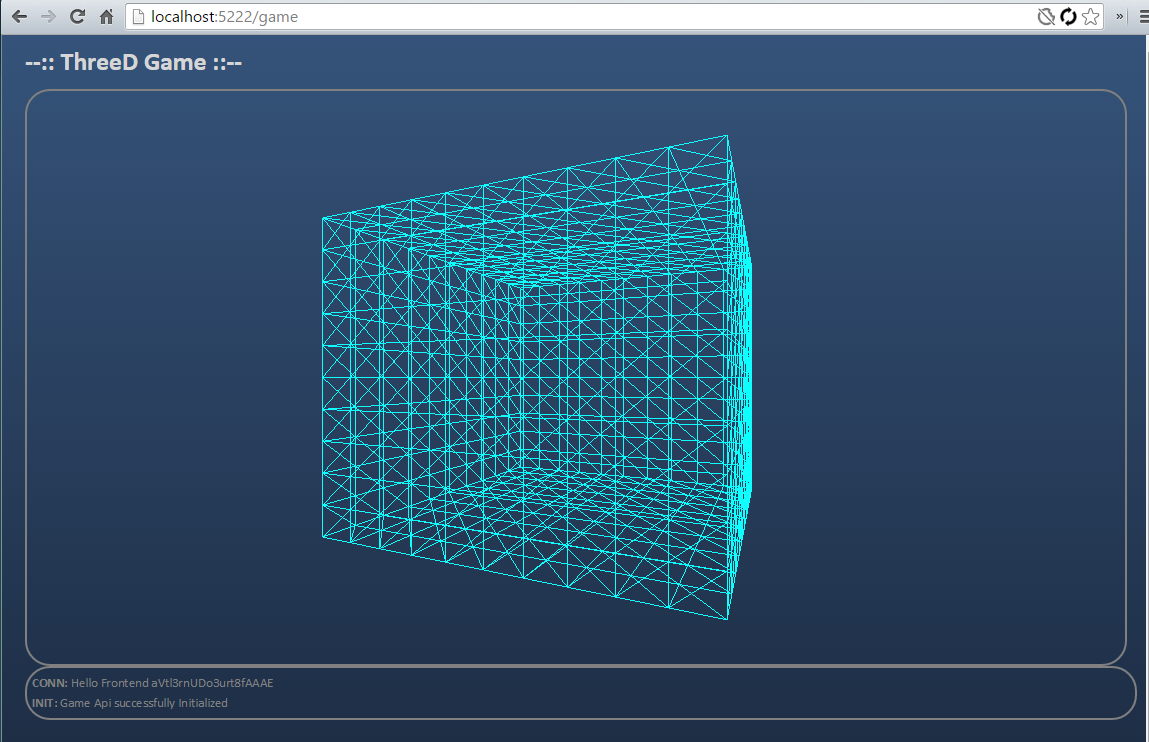
\includegraphics[width=10cm]{./images/FrontendInit.png}}
		\caption{Virtuelle Maschinen vs. Docker Container\cite{dockercontainer}}
		\label{fig:dockerVM}
\end{figure}
\subsubsection{Hardware}
Smartphone Controller, Platformunabhängig Node Server

%
% -----------------Implementation-------------------------
%

\section{Implementation}
\subsection{Server and Networking}
\paragraph{Aufbau des Gesamtpakets}
Diagramm, und Beschreibung des Aufbaus, Schnittstelle zum Frontend, Unterschiede unserer "Frontends" (logisch)
\paragraph{Structure and usage of express routing}\mbox{}\\
Beschreibung des Ruoting, Methodenlistings und Beispiele
\paragraph{Managing of clients}\mbox{}\\
AUth//Register/Ananymous

\paragraph{KismetClient-Paket}\mbox{}\\
Das KismetClient-Paket beinhaltet die Kommunikation mit dem Kismet-Server. Für die Kommunikation mit dem Server müssen die benötigten Protokolle mit den gewünschten Feldern bei diesem registriert werden. Danach werden automatisch Veränderungen an den Client gesendet und dieser muss diese auf Event-Basis auffangen und verarbeiten. Für die von uns benötigten Informationen, nutzt der Client die beiden Protokolle \enquote{SOURCE} und \enquote{CLISRC}. Die benötigten Felder werden in den Tabellen \ref{tab:src} und \ref{tab:cli} aufgezeigt.


\begin{table}[!h]
	\centering
	\begin{tabular}{ | p{.2\textwidth} | p{.5\textwidth} | }
		\hline 
		\rowcolor{blau} \multicolumn{2}{l|}{\textcolor{white}{\textbf{SOURCE}}}  \\ \hline
		uuid & Die eindeutige ID der Quelle \\ \hline
		username & Der Name der Quelle \\
		\hline
	\end{tabular}
	\caption{Benötigte Felder des SOURCE Protokolls}
	\label{tab:src}
\end{table}

\begin{table}[!h]
	\centering
	\begin{tabular}{ | p{.2\textwidth} | p{.5\textwidth} | }
		\hline
		\rowcolor{blau} \multicolumn{2}{l|}{\textcolor{white}{\textbf{CLISRC}}}  \\ \hline
		mac & Die MAC-Adresse des gefundenen Gerätes \\ \hline
		uuid & Die ID der Quelle, welche das Gerät gesehen hat \\ \hline
		lasttime & Timestamp der Sichtung \\ \hline
		signal\_dbm & Signalstärke des Geräts in DBM \\
		\hline
	\end{tabular}
	\caption{Benötigte Felder des CLISRC Protokolls}
	\label{tab:cli}
\end{table}


\subsection{Frontend Client and Login}
Zur Live-Evaluation der vom Kismet Client in die Datenbank geschriebenen Daten, wurde eine Webanwendung mit Hilfe des Webframeworks Meteor\footnote{https://www.meteor.com/} geschrieben. \\
Die Anwendung wertet die vom Kismet Client bereitgestellten Messdaten reaktiv aus und lässt sich in einem Standard Webbrowser anzeigen. 
Zur Ermittlung der Position eines Gerätes werden die gemessenen Signalstärken für jedes Gerät von den unterschiedlichen Drohnen miteinander verglichen. Dabei wird der gleitende Mittelwert zur dritten Periode pro Drohne berechnet (siehe Abbildung \ref{eqn:middle}), um mögliche Schwankungen in den Messungen zu behandeln. Wobei x\raise0.5ex\hbox{d}(t) für den Messwert zum Zeitpunkt t an Drogne d steht.
\\Da die Experimente ergeben haben, dass der gemessene dbm-Wert für ein Gerät geringer wird, je weiter man sich von der Quelle entfernt, kann so ermittelt werden, an welcher Drohne sich ein Gerät am nähesten befindet. \\
Die berechneten Mittelwerte werden verglichen und der höchste Mittelwert bezeichnet die Drohne, und damit auch die Position, an der ein Gerät am nähesten ist. Anschließend kann gezählt werden, an welcher Drohne sich wie viele Geräte befinden. Mit Hilfe dieser Anwendung lässt sich das Ausgangsproblem lösen. Platziert man an jeder Bar in der Einrichtung eine Drohne, kann diese Anwendung erkennen, wie viele Personen sich an den unterschiedlichen Bars befinden und darauf reagieren, indem auf einem Fernseher Ermäßigungen für eine weniger besuchte Bar angeboten werden.
\begin{figure}
\begin{equation}
  \boxed{{ m }_{ MA }^{ d }(t) = \frac { 1 }{ 3 } \sum _{ i=0 }^{ 2 }{ { x }^{ d }(t-i) }}
\end{equation}
\caption{Gleitender Mittelwert zur dritten Periode}
\label{eqn:middle}
\end{figure}

\subsubsection{Client Connections}
Lorem ipsum dolor sit amet, consetetur sadipscing elitr, sed diam nonumy eirmod tempor invidunt ut labore et dolore magna aliquyam
\subsubsection{Eventlisteners}
Lorem ipsum dolor sit amet, consetetur sadipscing elitr, sed diam nonumy eirmod tempor invidunt ut labore et dolore magna aliquyam
\subsubsection{Object Preparations}
Lorem ipsum dolor sit amet, consetetur sadipscing elitr, sed diam nonumy eirmod tempor invidunt ut labore et dolore magna aliquyam
\subsubsection{Styles}


\subsection{GameAPI}
Zur Live-Evaluation der vom Kismet Client in die Datenbank geschriebenen Daten, wurde eine Webanwendung mit Hilfe des Webframeworks Meteor\footnote{https://www.meteor.com/} geschrieben. \\
Die Anwendung wertet die vom Kismet Client bereitgestellten Messdaten reaktiv aus und lässt sich in einem Standard Webbrowser anzeigen.
Zur Ermittlung der Position eines Gerätes werden die gemessenen Signalstärken für jedes Gerät von den unterschiedlichen Drohnen miteinander verglichen. Dabei wird der gleitende Mittelwert zur dritten Periode pro Drohne berechnet (siehe Abbildung \ref{eqn:middle}), um mögliche Schwankungen in den Messungen zu behandeln. Wobei x\raise0.5ex\hbox{d}(t) für den Messwert zum Zeitpunkt t an Drogne d steht.
\\Da die Experimente ergeben haben, dass der gemessene dbm-Wert für ein Gerät geringer wird, je weiter man sich von der Quelle entfernt, kann so ermittelt werden, an welcher Drohne sich ein Gerät am nähesten befindet. \\
Die berechneten Mittelwerte werden verglichen und der höchste Mittelwert bezeichnet die Drohne, und damit auch die Position, an der ein Gerät am nähesten ist. Anschließend kann gezählt werden, an welcher Drohne sich wie viele Geräte befinden. Mit Hilfe dieser Anwendung lässt sich das Ausgangsproblem lösen. Platziert man an jeder Bar in der Einrichtung eine Drohne, kann diese Anwendung erkennen, wie viele Personen sich an den unterschiedlichen Bars befinden und darauf reagieren, indem auf einem Fernseher Ermäßigungen für eine weniger besuchte Bar angeboten werden.
\begin{figure}
\begin{equation}
  \boxed{{ m }_{ MA }^{ d }(t) = \frac { 1 }{ 3 } \sum _{ i=0 }^{ 2 }{ { x }^{ d }(t-i) }}
\end{equation}
\caption{Gleitender Mittelwert zur dritten Periode}
\label{eqn:middle}
\end{figure}

\subsection{Demonstration}
\subsubsection{Preparations}
\begin{enumerate}
 \item Ein Computer ist als Kismet-Server sowie als Meteor Server konfiguriert.
 \item Die Raspberry Pis, die als Kismet Drohnen konfiguriert sind, werden an die entsprechenden Positionen platziert, an denen die Anzahl der Geräte gemessen werden soll. Im Anwendungsfall dieses Projekts wird eine Drohne jeweils an einer Bar platziert. 
 \item Die Drohnen werden per LAN - Kabel an das Netzwerk verbunden, in dem sich auch der Kismet-Server befindet.
\end{enumerate}
\subsubsection{Start applications}
\begin{enumerate}
 \item Der Kismet-Server wird mit dem Befehl \emph{sudo kismet} über den Terminal gestartet.
 \item Die Meteor Anwendung wird mit dem Befehl \emph{meteor} über den Terminal gestartet. Die Mongo Datenbank wird dabei automatisch mit gestartet.
 \item Der Kismet Client wird mit Hilfe des Java Archives gestartet. Als Parameter können beim Start über den Terminal die IP - Adressen und Ports des Kismet-Servers und der Mongo Datenbank übergeben werden, sollten diese von den Standardkonfigurationen abweichen.
\end{enumerate}
\subsubsection{Running}
\begin{enumerate}
 \item Der Kismet-Server gibt im Terminal Statusnachrichten zu den Drohnen und gefundenen Netzwerken aus.
 \item Die Meteor Anwendung kann über einen Browser aufgerufen werden. \emph{[IPDesMeteorServers]:3000}
 \item Die Mongo Datenbank kann über den Befehl \emph{meteor mongo} im Terminal aufgerufen werden.
 \item Der Kismet Client gibt im Terminal Statusnachrichten zu den Informationen, die gespeichert werden aus.
\end{enumerate}

\section{Results}\label{result}
\subsection{Measurements}


\begin{figure}[H]
\begin{minipage}[t]{0.4\textwidth}
\vspace{0pt}
\paragraph{Structure}\mbox{}\\
Im Masterlabor wurde die ersten Probemessung durchgeführt, um zu testen, ob eine Positionsbestimmung durch Vergleichen der Dämpfungswerte überhaupt möglich ist. Dazu wurden zwei Drohnen an verschiedenen Enden des Raumes platziert. Bei der Messung wurde eine App benutzt die sekündlich einen Broadcast nach Access Point durchführt. Dadurch wird traffic generiert, der nötig ist, damit die Drohnen genug Pakete abfangen.
\end{minipage}
\hfill
\begin{minipage}[t]{0.5\textwidth}
\vspace{0pt}
\centering
		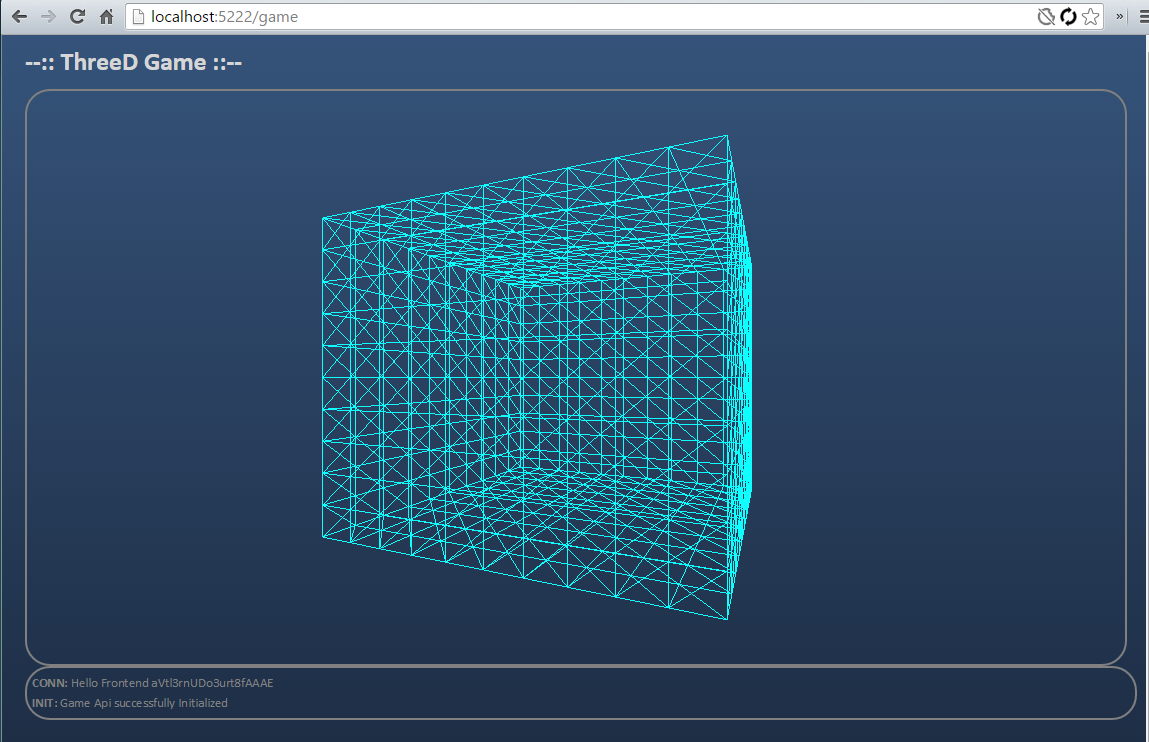
\includegraphics[height=5cm]{./images/FrontendInit.png}
		\caption{Probemessung}
		\label{fig:probeMessung}
\end{minipage}
\end{figure}

\paragraph{Ablauf der Messung}\mbox{}\\
Anschließend wurde die in Abbildung \ref{fig:probeMessung} zur erkennende Strecke mit einem Smartphone abgelaufen. Beim Abgehen der Strecke wurde nach circa jedem Meter eine kurze Zeit verweilt, damit ein aussagekräftigeres Ergebnis erzielt werden konnte.

\paragraph{Results}\mbox{}\\
Auf Abbildung \ref{fig:test1} ist zu sehen von welcher Drohne sich das Gerät entfernt und welcher es sich nähert.\\

\begin{figure}[H]
\begin{minipage}[t]{0.4\textwidth}
\vspace{0pt}
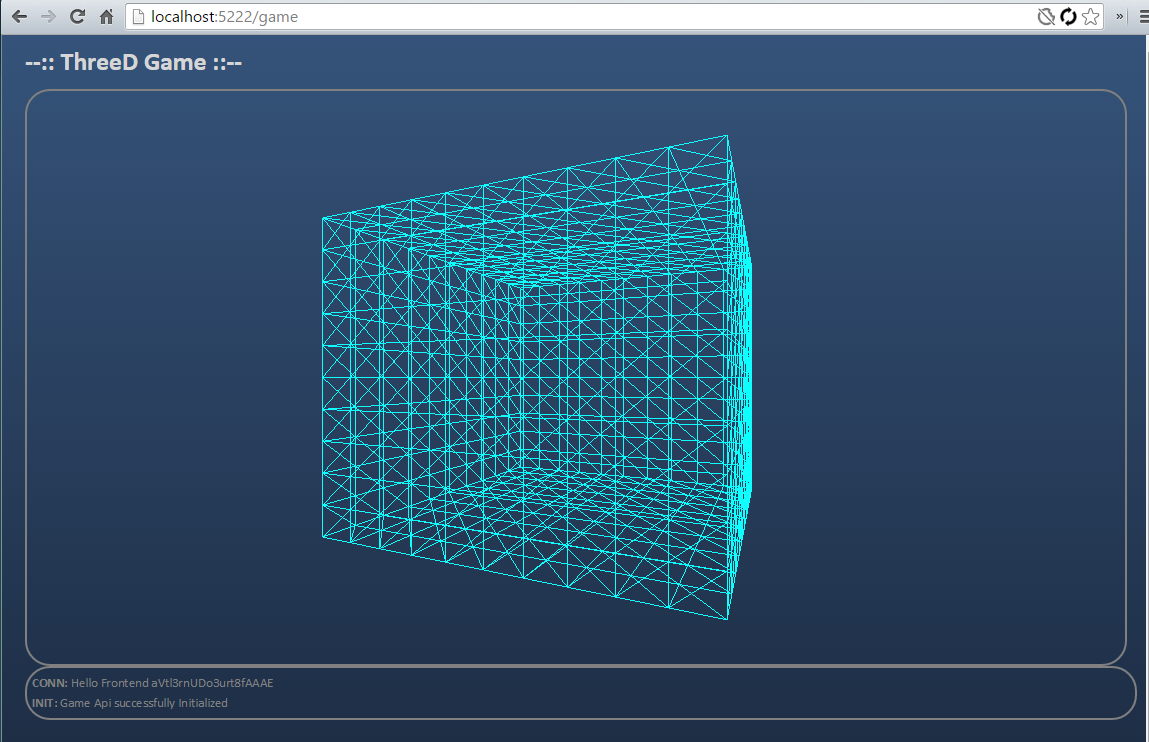
\includegraphics[height=5cm]{./images/FrontendInit.png}
\caption{Berechnungen zum Ergebnis}
\label{fig:tablleMessung}
\end{minipage}
\hfill
\begin{minipage}[t]{0.5\textwidth}
\vspace{0pt}
		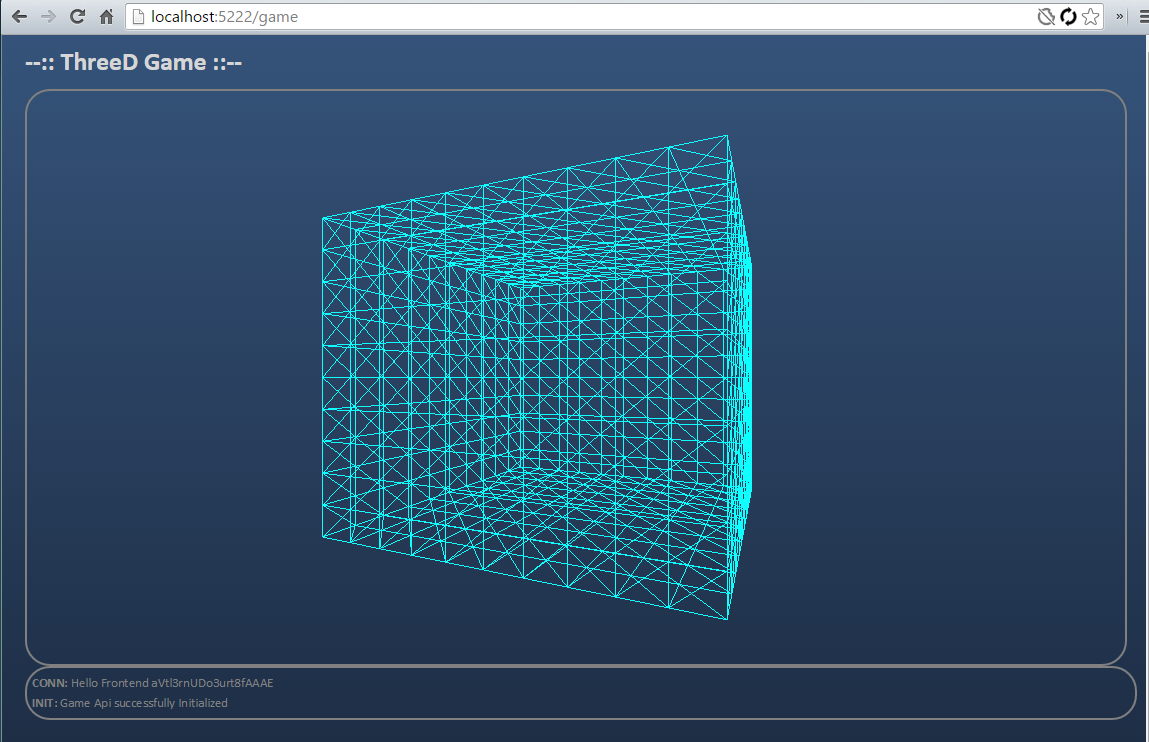
\includegraphics[width=\textwidth]{./images/FrontendInit.png}
		\caption{Ergebnis der Probemessung}
		\label{fig:test1}
\end{minipage}
\end{figure}

\subsection{Limitations}
\subsubsection{1. Test}

\paragraph{Ergebnis}\mbox{}\\
Selbst auf kurzer Distanz ist eine Differenz von ca. 10 dBm zwischen den Messpunkten zu sehen. Dies ermöglicht eine Ortsbestimmung auf kurzer Distanz, was beim nächsten Test ebenfalls zu sehen ist.

\begin{table}[H]
\centering
	\begin{tabular}{ | p{2.5cm} | l | l | l | }
		\hline 
		Entfernung	& 50 cm	& 100 cm	& 200 cm	\\ \hline
		Durchschnittliche Dämpfung & -62,22 dBm	& -75,45 dBm	& -82,52 dBm \\
		\hline
	\end{tabular}
	\caption{Ergebnisse des 1. Tests im störungsfreien Raum}
	\label{tab:probeTab}
\end{table}

\subsubsection{2. Test}\label{testNr2}

\begin{figure}[H]
\begin{minipage}[t]{0.4\textwidth}
\vspace{0pt}
\paragraph{Aufbau}\mbox{}\\
Um zu ermitteln, wie genau der Vergleich von Dämpfungswerten für die Positionsermittlung benutzt werden kann, wurden zwei Kismet-Drohnen in 12 Meter Abstand voneinander aufgestellt. Diese waren über einen Switch mit dem Kismet-Server verbunden. Alle 120 cm wurde ein Messpunkt festgelegt. Dies entsprach der Größe einer Bodenplatte im störungsfreien Raum und wurde deshalb als Distanz gewählt.
\end{minipage}
\hfill
\begin{minipage}[t]{0.5\textwidth}
\vspace{0pt}
		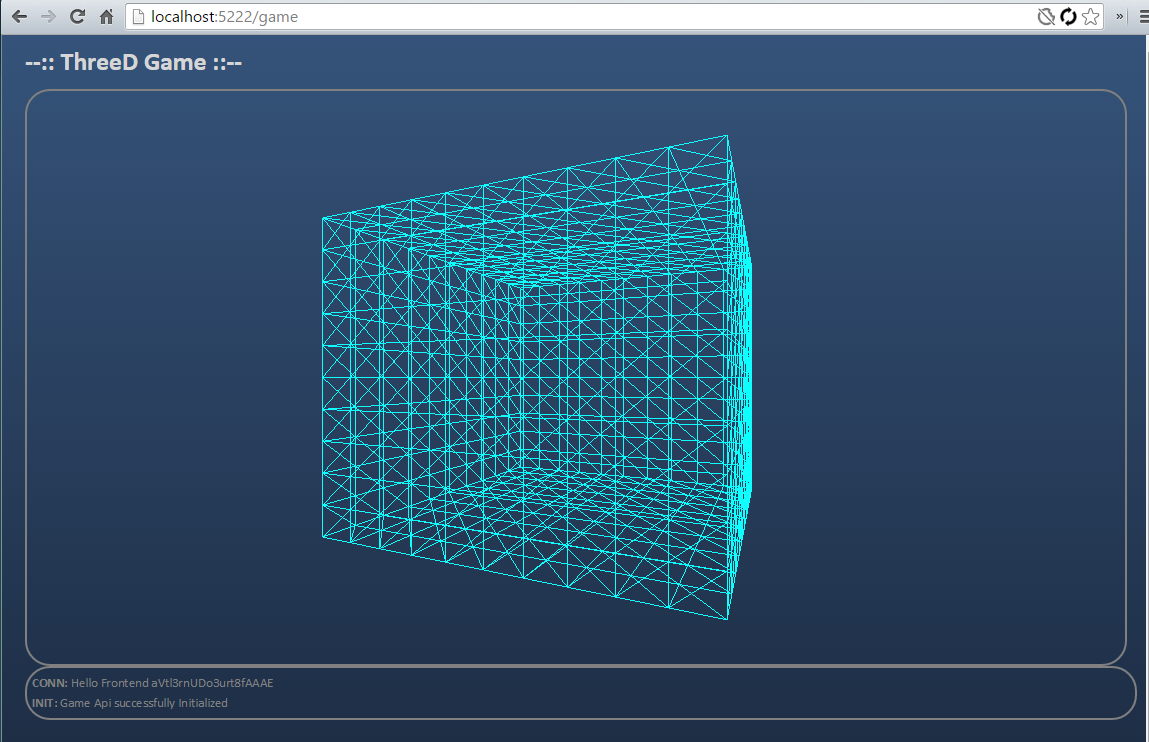
\includegraphics[width=\textwidth]{./images/FrontendInit.png}
		\caption{Aufbau 2. Test Störungsfreier Raum}
		\label{fig:test2}
\end{minipage}
\end{figure}

\paragraph{Ablauf der Messung}\mbox{}\\
Ein Smartphone wurde auf den entsprechenden Messpunkt gelegt. WiFi war auf dem Gerät eingeschaltet und die App zur Traffic-Generierung war aktiv. Es wurden pro Messpunkt circa 100 Messwerte aufgenommen, damit eine aussagekräftiges Ergebnis erzielt werden konnte und kurzzeitige Störungen abgefangen werden konnten.

\paragraph{Ergebnis}\mbox{}\\
Wie schon bei der ersten Probemessung ist eine deutliche Tendenz zu erkennen. Bei der Drohne, von der sich das Smartphone entfernte, nahm die Dämpfung zu. Bei der anderen Drohne nahm sie ab. Die aufgenommen Dämpfungswerte sind bei circa 480 cm gleich groß (siehe Diagramm \ref{fig:480} im Anhang). Dies ist 120 cm von der eigentlichen Mitte entfernt. Somit besteht eine Messungenauigkeit von 120 cm.

\subsection{Realistische Messung}
\paragraph{Aufbau}\mbox{}\\
Der Aufbau der Messung war der gleiche wie in der 2. Messung im störungsfreien Raum (siehe \ref{testNr2}). Dieses mal fand die Messung allerdings in einem einfachen Flur der FH-Kiel statt und war somit nicht vor Störungen geschützt.

\paragraph{Ablauf der Messung}\mbox{}\\
Ein Smartphone wurde an den einzelnen Messpunkten platziert. Das WiFi war auf dem Gerät aktiviert. Allerdings war das Gerät mit keinem WiFi-Netzwerk verbunden um die realen Umstände in einer Discothek nachempfinden zu können. Da von Anfang an festgestellt wurde, dass deutlich weniger Pakete abgefangen wurden, wurde die Dauer der Messung an jedem Messpunkt auf 2 Minuten festgesetzt.

\paragraph{Ergebnis}\mbox{}\\
Zu beobachten war, dass in den 2 Minuten 3-9 Pakete abgefangen wurden. Das macht eine Echtzeit-Bewegungsverfolgung so gut wie unmöglich. Ebenso war die Differenz der gemessenen Dämpfungswerte geringer, was eine Positionierung des Geräts erschwert. Das liegt daran, dass auf dem Flur Strahlen der WiFi-Antenne des Smartphones weniger stark gedämpft wurden. 


\section{Conclusion}
Eine passive Ortung von WiFi-Geräten anhand der Signalstärke ist möglich. Eine Installation einer zusätzlichen Anwendung auf den zu ortenden Geräten ist nicht notwendig. Es ist zu beachten, dass durch die starken Schwankungen in der Signalstärke nur eine  Positionsbestimmung auf 1,2 Meter möglich ist (siehe Diagramm \ref{fig:480} im Anhang).
\\
Ein weiteres Forschungsfeld ist die zeitliche Genauigkeit der bestimmten Position. Da nur unregelmäßig und nicht vorhersagbar Daten eingehen ist eine Echtzeitortung nicht trivial und bedarf weiterer Untersuchung.
Die in dieser Arbeit vorgestellte Technologie eignet sich für die Raum bezogene Ortung von Geräten. 
\\
Rechtliche Rahmenbedingen sind bei der vorgestellten Positionsbestimmung einzuhalten. Es ist zu klären, in wie weit die MAC-Adresse eines Gerätes unter Datenschutzbestimmungen fällt.
\\
In einer zukünftigen Weiterentwicklung kann versucht werden die genaue Position des Gerätes über Triangulation zu bestimmen. Es ist möglich aus den erfassten Daten die Position zu berechnen, solange es mindestens drei Messtationen gibt. Einige Schwierigkeiten dabei sind zum Beispiel Objekte im Messbereich, Wände sowie Personen. Diese verändern die Signalstärken und müssen im Algorithmus berücksichtigt werden. Dies führt zu einer weiteren nicht einfach zu lösenden Problemstellung welche die Aufstellung des Algorithmus abdeckt. \linebreak
\linebreak
Im Weiteren kann die Positionsbestimmung über eine Fingerprint-Map durchgeführt werden. Hierbei ist ein genaueres Ergebnis zu erwarten als bei der Berechnung mittels der Triangulation. Dies liegt an der leichteren Berücksichtigung von starren Objekten in dem Messgebiet. Der Nachteil liegt in der vorherigen Aufstellung der Karte. Für diese muss das Gebiet vermessen worden sein, um eine Datenbank mit Signalstärken aufzustellen. 
\linebreak
Eine weitere Erforschung sollte beide Ansätze in Betracht ziehen und kombinieren, um die genaue Position des Nutzers bestimmen zu können.


\newpage
%%%%%%%%%%%%%%%%%%%%%%%%%%%%%%%%%%%%%%%%%%%%%%%%%%%%%%%%%%%%%
%%%%% References %%%%%
\bibliographystyle{spiebib}   %>>>> makes bibtex use spiebib.bst
\bibliography{references}   %>>>> bibliography data in report.bib

\newpage
\appendix
\section{Outlook} \label{subsection:Einlasskontrolle}
\subsection{Anforderungsanalyse}
Die Einlasskontrolle ist in Meteor entwickelt. Eine Anforderungsanlyse mit Diskothekenbesitzern ergab folgende Anforderungen:

\begin{itemize}
\item Gäste können sich auf eine Gästeliste über eine Micro-Event-Page setzen (bereits existent in einer Java-Anwendung)
\item Gäste bekommen bei der Anmeldung auf der Gästeliste eine E-Mail mit einem QR-Code zugesendet
\item Gäste werden in einer Liste für jedes Event angezeigt
\item In der Liste können Gäste durch anklicken eingechecked werden
\item Gäste können alternativ über einen QR-Code-Scanner eingechecked werden
\item Checkins werden in einem Diagramm zusammengefasst
\end{itemize}
\subsection{Konzept und Implementierung}
Als Framework wird Meteor eingesetzt. Über eine API wird bei jeder Anmeldung von einem Gast auf der Gästeliste der Gast an die Meteor-Anwendung übertragen.
Bei einem Checkin wird der neue Status von der Meteoranwendung an die bestehende Java-Anwendung übertragen.
\\
Der an den Gast via E-mail gesendete QR-Code enthält eine per Java generierte einmalige ID (UUID), welche mit der Gast-Anmeldung für ein Event verknüpft ist.
\\
Für den Scanvorgang wird das Framework jsqrcode in Meteor eingebunden. Der Eventhandler qrScanner.on('scan') wird jede Sekunde gefeuert. In der Callback-Funktion wird die Variable messages zurückgegeben. Ist diese nicht null, enthält sie den Wert des QR-Codes, welcher zum Checkin verwendet wird.


\subsection{Ausblick}
Die Einlasskontrolle kann wie folgt mit dem Indoor-Tracking verbunden werden, um Personen in einem Raum zu orten:
\begin{enumerate}
\item Eine Person wird über einen QR-Code erkannt.
\item Das stärkste Signal von Smartphone (MAC) wird erkannt.
\item Die MAC-Addrese wird der Person zugeordnet.
\item Das Smartphone beziehungsweise die Person wird im Raum erkannt.
\end{enumerate}

\section{Ergebnisse der Messungen im störungsfreien Raum}\label{testAnhang}
Hier sind die Messergebnisse des 2. Tests aus dem störungsfreien Raum zu sehen. Es ist zu beobachten, dass sich die Linien der beiden Drohnen annähern und dann wieder auseinander driften. Beim Diagramm \ref{fig:480} sind die Dämpfungswerte etwa gleich groß, was auf einen Messungenauigkeit von 1,2 Metern schließen lässt, da der eigentliche Mittelpunkt bei 600 cm liegt.

\begin{figure}[H]
	\centering
	%	\fbox{\includegraphics[width=16cm]{./images/120cm.png}}
		\caption{Messergebnis beim 120 cm}
		\label{fig:120}
\end{figure}




\end{document} 
